\chapter{Diversiteit in game content}
De corporate learning afdeling van \&ranj houdt zich vooral bezig met het maken van narrative games op maat. Er is een ontwikkelomgeving opgezet waarin narrative games efficiënter ontwikkelt kunnen worden. In dit hoofdstuk wordt er ingezoomd op de story- en dialog editor, waarin het narratief achter het spel geschreven kan worden zonder enige programmeerkennis. 
De huidige editors moeten telkens aangepast worden om met de diversiteit aan game content om te kunnen gaan die de projecten op maat introduceren. Dit hoofdstuk stelt een oplossing voor waarmee de editors op een flexibele manier om kunnen gaan met het verschil in game content.

\section{Story- en dialog editor}
Tijdens het ontwikkelproces van een narrative game werken game designers, visual designers en programmeurs nauw samen. Om game designers het verhaal te laten schrijven en hierin visuals te tonen zijn er twee editors opgezet; de story- en dialog editor. De programmeurs kunnen vervolgens de game engine aanpassen om de data van de editors te interpreteren, om zo het verhaal te visualiseren in het spel.
Game designers maken gebruik van de visual scripting interface die de editors bieden. Deze visual scripting interface bestaat uit visuele componenten, ook wel nodes of vertices genoemd, die op een canvas geplaatst kunnen worden. Vervolgens kunnen er verbindingen, edges, worden gelegd tussen deze vertices. De gehele datastructuur met vertices en edges wordt een graph, of in het Nederlands graaf, genoemd\cite{Aho1983}. Deze datastructuur is goed terug te zien in de editors. Een voorbeeld hier van is \autoref{fig:storyeditorsimplegraph}

\begin{figure}[htb]
    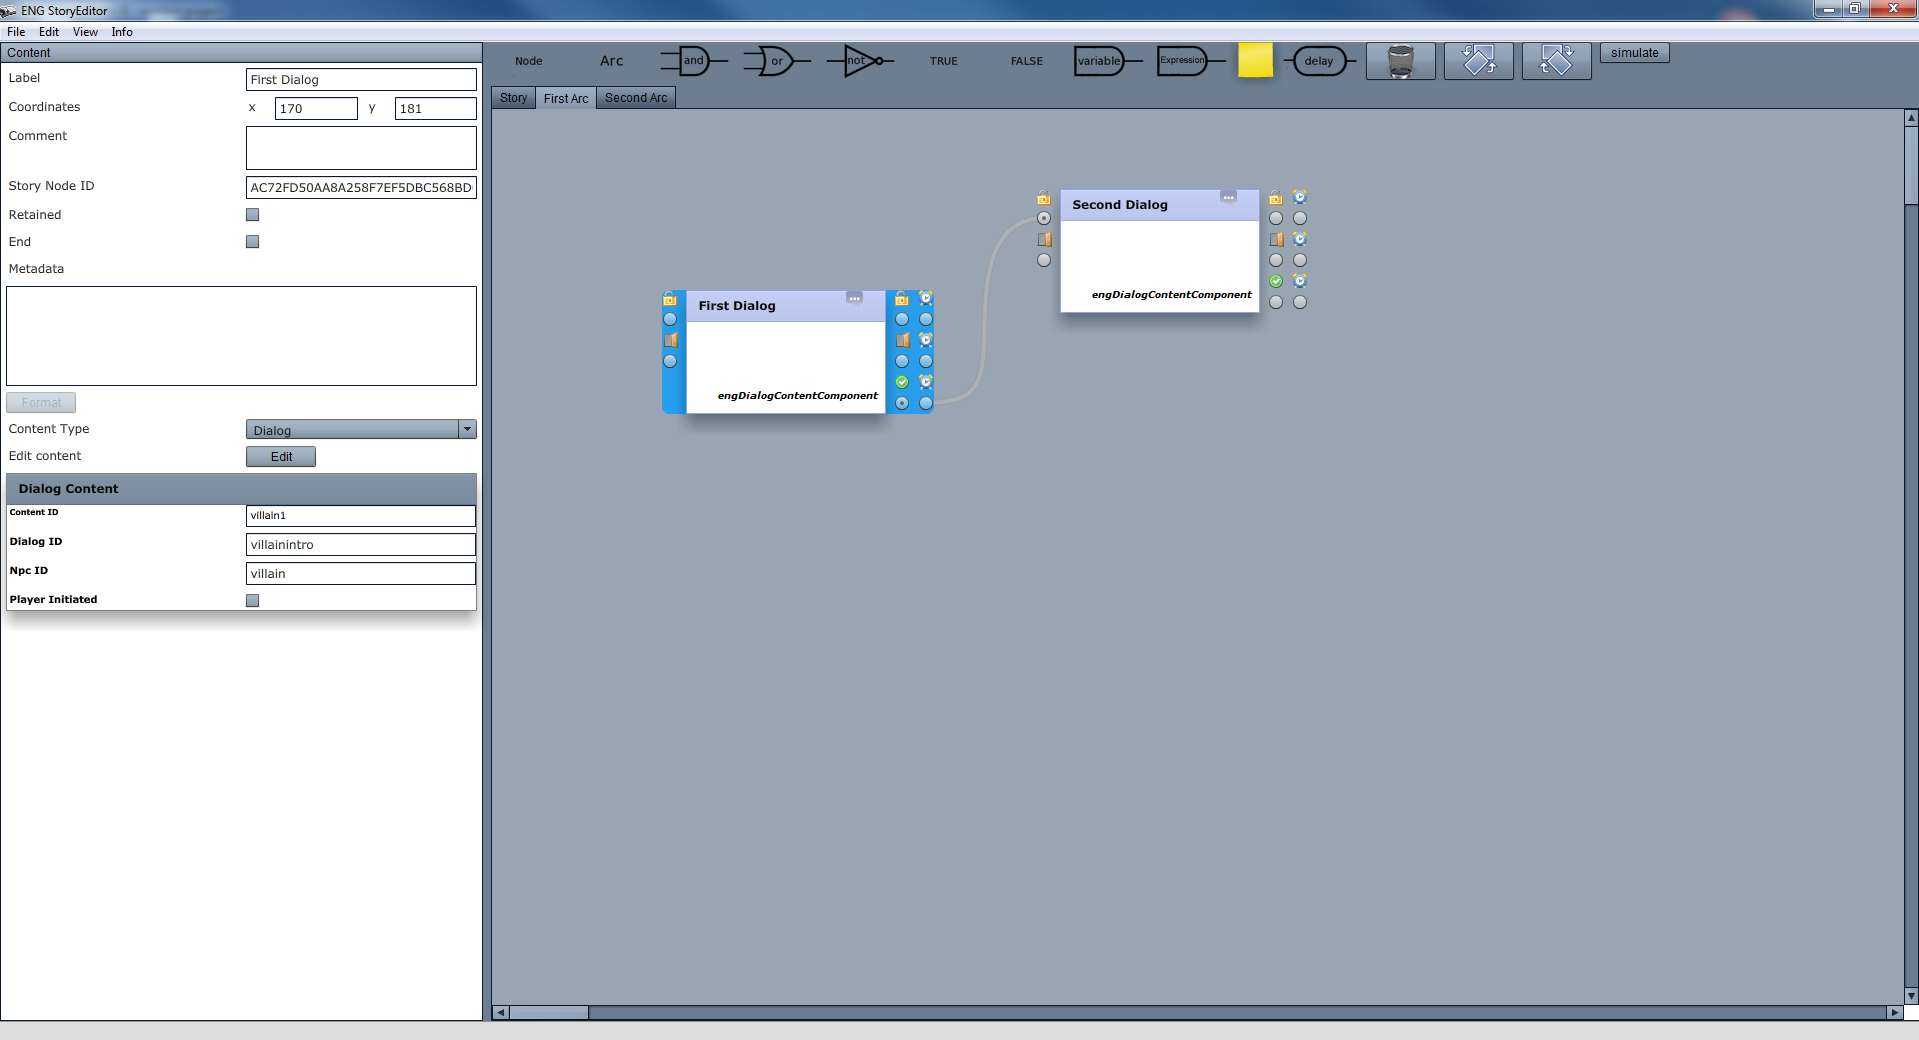
\includegraphics[width=\textwidth,height=\textheight,keepaspectratio]{StoryEditor_SimpleStory_2dialogs}
    \caption{Een simpel verhaal gemaakt in de story editor}
    \label{fig:storyeditorsimplegraph}
    \centering
\end{figure}

\section{Content typen}
Om onderscheid te kunnen maken tussen nodes maken de editors gebruik van een gespecialiseerde nodes genaamd: content node. Deze nodes bevatten een content type; een stukje game content. Denk hierbij aan een dialog, tekst of afbeelding. Ieder content type heeft een eigen betekenis en doel. In \autoref{fig:storyeditorsimplegraph} wordt er gebruik gemaakt van ‘dialog content’ nodes die een dialoog starten. Een ander voorbeeld van een content type is een ‘text content’ node, deze kan als doel hebben om tekst te tonen. Verder bevatten content types ‘properties’. Dit zijn velden die verdere informatie geven over de eigenschappen van het doel. Zo heeft het content type ‘text content’ een property genaamd ‘Text' wat de tekst is die getoond zal worden door ‘text content’. Een content type is dus een datastructuur met een betekenis in de game. Door middel van content typen wordt er semantiek gebonden aan content nodes.
Door de semantische eigenschappen van een content node kunnen zowel de game designers als programmeurs onderscheid maken tussen de nodes. Programmeurs schrijven code om deze content types af te vangen en te interpreteren. Als er geen onderscheid bestaat weet de game engine niet wat er getoond moet worden wanneer er een content node vrijkomt.
Echter hebben de meeste content typen een vrij impliciet doel. Zo kan ‘text content’ een tekst bevatten die uitgesproken wordt door een karakter in het verhaal, maar het kan ook een mogelijk antwoord zijn dat de speler kan geven op een vraag. Om duidelijk onderscheid te maken is het belangrijk dat content typen zo expliciet mogelijk zijn in hun doel. Dit leidt naar content typen zoals ‘answer content’ en ‘quiz content’. Het is belangrijk dat er weinig ruimt is voor verschillende interpretaties.

\subsection{Vervuiling van de scope}
Een nadeel van content typen met een expliciet doel is dat ze meestal maar bruikbaar zijn voor een enkel project. Vooral in projecten waarin game content erg van elkaar verschild is dit een probleem, hergebruik van content typen is erg laag. Per project worden er nieuwe content types aangemaakt, omdat de game content niet overeenkomt met vorige projecten. Echter kunnen al bestaande content typen niet worden verwijderd uit de editors, omdat de editor dan niet meer gebruikt kan worden voor oudere projecten. Dit alles zorgt voor een vervuiling van de content typen scope; content typen zijn beschikbaar in project die ze niet benutten.

\pagebreak

\subsection{Statische definities}
\begin{wrapfigure}{r}{0.4\textwidth}
    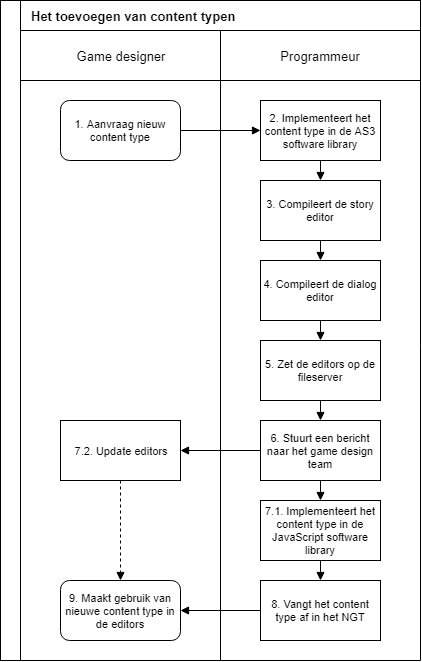
\includegraphics[width=0.38\textwidth]{Proces_ToevoegenContentTypeHuidig}
    \caption{Proces: het toevoegen van content types}
    \label{fig:procesaddcontenttypescurrent}
    \centering
\end{wrapfigure}
De editors maken gebruik van content types die gedefinieerd zijn in de \&ranj software library. In de software library bevinden zich klassen die ieder een content type vormt; content types hebben een statische definitie, ze zijn in de editor gebakken. Dit biedt wel meer controle over het content type, maar deze hoeveelheid controle overtollig, content types blijven datastructuren. Hiernaast maakt dit het proces van het toevoegen en verwijderen van content types lastiger. Om dit te bereiken moet de broncode van de editor worden aangepast en vervolgens moet de editor opnieuw worden gecompileerd. Het huidige proces voor het toevoegen van een content type ziet eruit als in \autoref{fig:procesaddcontenttypescurrent}.

\begin{enumerate}
    \item De game designer wilt onderscheid maken tussen quiz tekst die gebonden staat aan een tijdslimiet en vragen die de hoofdpersoon zichzelf stelt, waarbij de speler geen tijdsdruk heeft. Hij of zij heeft aparte content typen nodig om onderscheid te maken tussen deze twee typen game content.
    \item De programmeur implementeert deze content typen in de \&ranj ActionScript3 (AS3) software library. Uit deze library halen de editors de content types. In de software library wordt aan gegeven welke editors gebruik mogen maken van het content type. Hieruit kan geconcludeerd worden dat er geen encapsulatie van content typen bestaat. De editors zouden zelf aan moeten geven van welke content typen ze gebruik maken.
    \item De programmeur haalt de nieuwe versie van de AS3 library binnen en past het versie nummer aan. Hij of zij compileert handmatig de story editor. Hierna wordt er “clone” achter de applicatie sleutel (application identifier) geplakt en de story editor voor de tweede keer gecompileerd. Dit maakt het openen van twee story editor schermen mogelijk. Anders kunnen er geen twee instanties van Apache Flex applicaties tegelijk openstaan.
    \item Stap 3 wordt herhaald door de programmeur, maar dan voor de dialog editor.
    \item De installers van de vier editors worden op de file server van \&ranj gezet. Dit is een gedeelde folder waar medewerkers van het bedrijf toegang tot hebben.
    \item De programmeur stuurt een mail naar het game design team waarin staat dat er een nieuwe versie van de editors beschikbaar is. Hiernaast staan veranderingen en de locatie van de nieuwe editor in de mail.
    \item Terwijl de game designers de editors updaten (7.2), implementeert de programmeur het content type in de JavaScript software library, zodat deze gebruikt kan worden in het NGT.
    \item De programmeur vangt het nieuwe content type af in het NGT en linkt deze aan de correcte actie.
    \item De game designer kan gebruik maken van het nieuwe content type. De game interpreteert het content type.
\end{enumerate}

\noindent De programmeur moet eerst de Apache Flex editor projecten opgezet hebben en daarnaast kennis hebben van deze projecten. Hiernaast moet de editor handmatig getest worden na het toevoegen van de nieuwe content typen om te kijken of er per ongeluk niks gebroken is. Dit kan kostbare tijd en geld kosten.
Een geautomatiseerde deployment pipeline zou kunnen helpen en veel werk uithanden nemen van de programmeur. Hiernaast moet het compilatie en deployment proces zoveel mogelijk vermeden worden, omdat dit tijd kost. Content typen blijven datastructuurtjes en het toevoegen of aanpassen van deze structuren zou geen compilatie van beide editors moeten vereisen.

\subsection{Misbruik van content types}
Omdat het toevoegen of aanpassen van content typen een langdradig proces is wordt dit het liefst vermeden. Vaak worden er content typen uit oudere project misbruikt om onderscheid te kunnen maken tussen game content. Zo wordt ‘MinigameContent’ regelmatig gebruikt voor het tonen van hele andere dingen dan minigames.
Door content typen bij projecten op verschillende manieren te gebruiken kan er nooit op de eerste blik zeker gezegd worden wat voor doel het content type heeft.

\section{Dataschema’s}
Vanwege de diversiteit in game content verschillen de content typen sterk per project. De selectie aan content types wordt geacht om dynamisch te zijn. Echter staan deze statisch gedefinieerd in de \&ranj AS3 software library. Er moet een manier komen om per project een selectie aan content typen te kunnen specificeren.
Een content type is een (kleine) datastructuur die bestaat uit een aantal velden. Zo bestaat ‘sms content’, een content type die een SMS vrij laat komen, uit een afzender, datum en inhoud. Door in ActionScript3 een type aan een veld toe te kennen kan er worden afgedwongen dat afzender en inhoud een tekst zijn en dat de datum een datum is. Vervolgens verbiedt de user interface foutief gebruik; de datum moet in een correct formaat staan. Restricties opleggen aan de user interface als validatie is gevaarlijk, want het is nog steeds niet zeker of de data valide is omdat deze mogelijk ook op andere manier kan ontstaan. Er wordt dus gezocht naar een oplossing waarmee velden in een content type gespecificeerd kunnen worden. Hiernaast moeten deze velden gevalideerd kunnen worden.

\begin{wrapfigure}{r}{0.5\textwidth}
    \fbox{
        \parbox{0.48\textwidth}{
            \textbf{SMSContent} bestaat uit\\
            een \textbf{afzender} weergeven in \textbf{tekst}\\
            een \textbf{ontvang datum} weergeven als \textbf{datum}\\
            een \textbf{inhoud} weergeven als \textbf{tekst}
        }
    }
    \caption{Pseudo dataschema voor 'sms content'}
    \label{fig:pseudosmscontent}
\end{wrapfigure}

\pagebreak
\noindent Om de velden van de content typen te specificeren zal er gebruik gemaakt worden van dataschema’s. Met dataschema’s kan er een set aan regels worden opgelegd aan de datastructuur. Hierbij is het belangrijk dat het zowel leesbaar is voor mens als machine. Een pseudo dataschema voor ‘sms content’ zou eruit kunnen zien als in \autoref{fig:pseudosmscontent}.
Dit pseudo dataschema is leesbaar voor mensen, maar niet voor computers. Computers hebben een gestandaardiseerd formaat nodig om data te kunnen interpreteren, zoals Extensible Markup Language (XML) of JavaScript Object Notation (JSON).
Door gebruik te maken van een dataschema kan het proces voor het toevoegen van content typen sterk worden versimpeld. Het nieuwe proces wordt weergeven in \autoref{fig:procesaddcontenttypesnew}.

\begin{figure}[htb]
    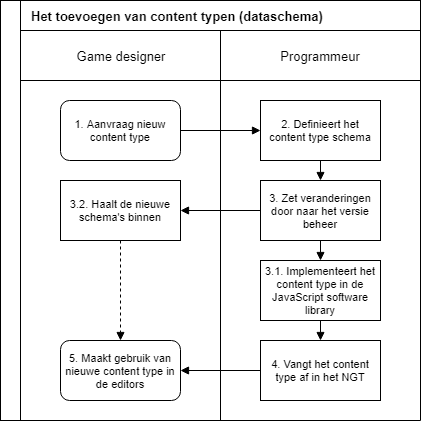
\includegraphics[width=\textwidth,height=\textheight,keepaspectratio]{Proces_ToevoegenContentTypeNieuw}
    \caption{Een versimpeld proces voor het toevoegen van content typen.}
    \label{fig:procesaddcontenttypesnew}
    \centering
\end{figure}

\subsubsection{XML-dataschema}
XML heeft dataschema functionaliteit; de onderliggende structuur van een XML-object kan worden gespecificeerd. Dit bereikt XML door middel van elementen en attributen. De eerder beschreven ‘sms content’ kan worden beschreven in een XML-dataschema als in \autoref{fig:xmlschemasmscontent}. Vervolgens kunnen XML-objecten gevalideerd worden door het schema. Het XML-object in \autoref{fig:xmlsmscontent} is valide, want de structuur komt overeen met die van het dataschema in \autoref{fig:xmlschemasmscontent}. JSON mist deze functionaliteit.

\begin{figure}[htb]
    \centering
    \lstset{
    language=XML,
    morekeywords={encoding,
        xs:schema,xs:element,xs:complexType,xs:sequence,xs:attribute}
    }
    \begin{lstlisting}
        <?xml version="1.0" encoding="UTF-8"?>
        <xs:schema xmlns:xs="http://www.w3.org/2001/XMLSchema">
            <xs:element name="smscontent">
                <xs:complexType>
                    <xs:sequence>
                        <xs:element name="sender" type="xs:string" />
                        <xs:element name="receiveDate" type="xs:dateTime" />
                        <xs:element name="content" type="xs:string" />
                    </xs:sequence>
                </xs:complexType>
            </xs:element>
        </xs:schema>                
    \end{lstlisting}
    \caption{XML-dataschema voor 'sms content'.}
    \label{fig:xmlschemasmscontent}
\end{figure}

\begin{figure}[htb]
    \centering
    \lstset{language=XML}
    \begin{lstlisting}
        <?xml version="1.0" encoding="UTF-8"?>
        <smscontent>
            <sender>Harold</sender>
            <receiveDate>2018-04-21T11:00:00</receiveDate>
            <content>Great moves, keep it up!</content>
        </smscontent>              
    \end{lstlisting}
    \caption{Valide XML-object van 'sms content'.}
    \label{fig:xmlsmscontent}
\end{figure}